\documentclass[tikz,border=2pt]{standalone}
\usepackage{amsmath,amssymb}
\usepackage{tikz}
\usetikzlibrary{arrows.meta}

\begin{document}
% The argument is the angle from the positive real axis, defined up to multiples of 2 pi;
% the principal value Arg z lies in (-pi, pi].
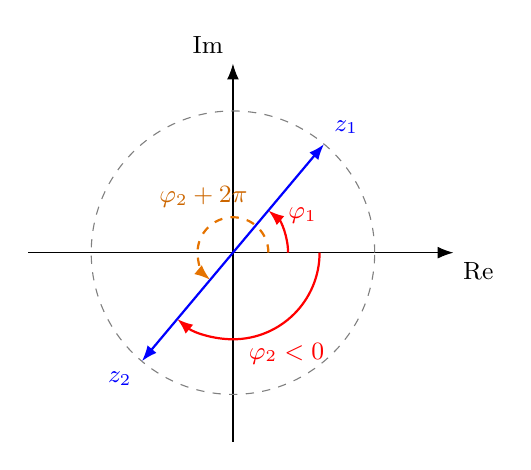
\begin{tikzpicture}[every node/.style={font=\small}, >={Latex[length=2mm]}]
	\draw[->] (-2.6,0) -- (2.8,0) node[below right] {$\mathrm{Re}$};
	\draw[->] (0,-2.4) -- (0,2.4) node[above left] {$\mathrm{Im}$};
	\draw[gray, dashed] (0,0) circle (1.8);
	\draw[->, blue, thick] (0,0) -- (50:1.8) node[above right] {$z_1$};
	\draw[red, thick, ->] (0.7,0) arc (0:50:0.7);
	\node[red] at (28:1.0) {$\varphi_1$};
	\draw[->, blue, thick] (0,0) -- (-130:1.8) node[below left] {$z_2$};
	\draw[red, thick, ->] (1.1,0) arc (0:-130:1.1);
	\node[red] at (-62:1.45) {$\varphi_2<0$};
	\draw[orange!90!black, thick, dashed, ->] (0.45,0) arc (0:230:0.45);
	\node[orange!80!black, font=\small] at (118:0.8) {$\varphi_2+2\pi$};
\end{tikzpicture}
\end{document}
